\documentclass[landscape, twocolumn, 12pt]{article}
\usepackage{TitlePage}

\usepackage{amsmath}
\usepackage{amssymb}
\usepackage{graphicx}
\usepackage{caption}
\usepackage{float}
\usepackage{pdfpages}
\usepackage{gensymb}
\usepackage{stanli}
\usepackage{tikz}
\usepackage{tikz-uml}

\everymath{\displaystyle}

\usepackage{hyperref}%Make references, clickable links
\hypersetup{
    colorlinks,
    citecolor=black,
    filecolor=black,
    linkcolor=black,
    urlcolor=black
}

%------------------------------------------------------------------------------------------
\newcommand{\ei}{\vec{e_1}}   %e1 shortcut
\newcommand{\ej}{\vec{e_2}}   %e2 shortcut
\newcommand{\ek}{\vec{e_3}}   %e3 shortcut
\newcommand{\n}{\vec{n}}
\newcommand{\m}{\vec{m}}
\newcommand{\x}{\vec{x}}

\newcommand{\sig}{\sigma}       %sigma shortcut
\newcommand{\ep}{\varepsilon} %epsilon shotcut

\renewcommand{\vec}[1]{\mathbf{#1}} %make vectors bold


\newcommand{\beq}{\begin{equation}} %begin equation shortcut
\newcommand{\eeq}{\end{equation}} %end equation shortcut

\newcommand{\of}[1]{\left(#1\right)} %parenthases shortcuts
\newcommand{\ofa}[1]{\left[#1\right]} %brackets shotcut

%%------------------------------
\usepackage{empheq}
\usepackage[most]{tcolorbox}
% Box commands
\newtcbox{\mymath}[1][]{%
    nobeforeafter, math upper, tcbox raise base,
    enhanced, colframe=blue!30!black,
    colback=blue!30, boxrule=1pt,
    #1}

\newcommand{\pbox}[1]{\begin{empheq}[box=\mymath]{align*}#1\end{empheq}} %purple box shortcut

% Reduce figure padding
\setlength{\intextsep}{2.0 pt plus 2.0pt minus 2.0pt}
\setlength{\belowcaptionskip}{-20pt}


% This provides the "strip" command which allows an equation to be one column.
% Note figures and tables can span both columns by adding a "*"
\usepackage{cuted}

%------------------------------------------------------------------------------------------
\begin{document}

%TITLE PAGE COMMANDS
	
\title{Structural Analysis with the Direct Stiffness Method}
\subtitle{Modeling Structural Systems as Springs}
\subject{CEE321}
\titleimage{Figures/TitlePageImage}
\author{Brian Chevalier}
\date{\today}
\maketitle
\pagenumbering{arabic}

\section{Truss Direct Stiffness Method}
\section{Beam Direct Stiffness Method}

A beam element has four degrees of freedom. Two degrees of freedom at each node which includes the rotation $\theta$ and the deflection or transverse displacement, $w$.

\begin{figure}[h]	\centerline{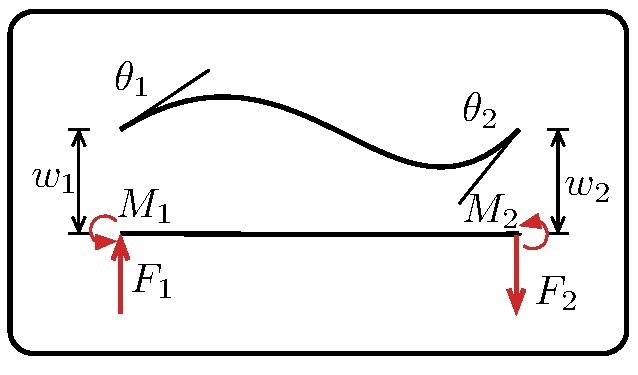
\includegraphics[width=0.7\columnwidth]{Figures/DeflectionandRotation}}
	\caption{Degrees of Freedom}
	\label{fig:DeflectionandRotation}
\end{figure}

\subsection{Bending Stiffness}

We will isolate each degree of freedom by applying boundary conditions at each node, such that each beam will only have one unrestrained kinematic unknown. Figure \ref{fig:BCFrame} shows the various boundary conditions that will be used to determine the beam bending stiffness. This will allow us to derive the force-displacement relationship necessary to solve the beam.

\begin{figure}[H]	\centerline{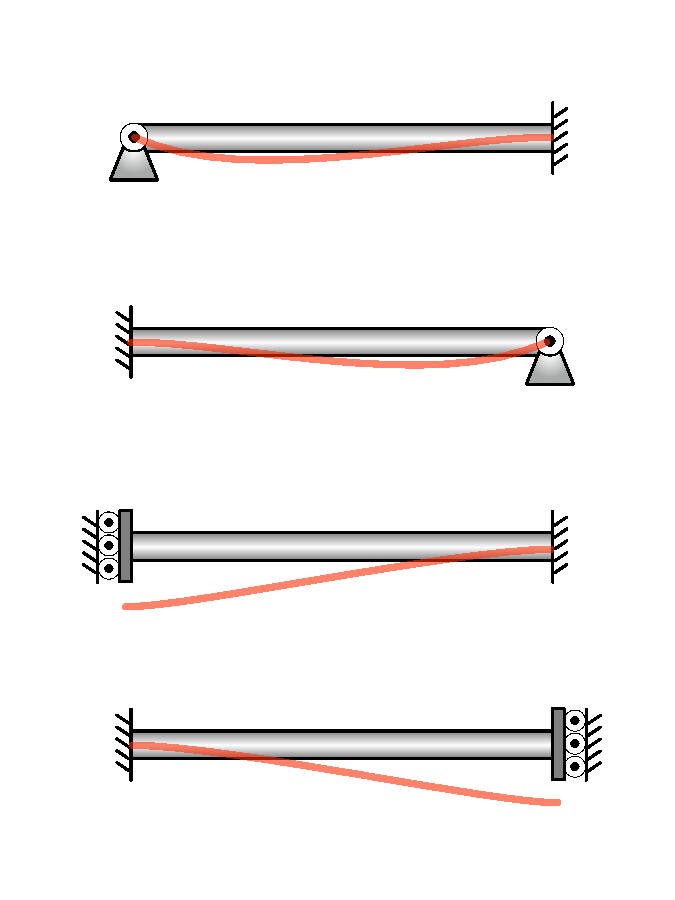
\includegraphics[width=0.9\columnwidth]{Figures/BCFrame}}
	\caption{Beam Boundary Conditions}
	\label{fig:BCFrame}
\end{figure}

\begin{align*}
	w_1=0 & \text{	} \theta_1=?\\
	w_2=0 &\text{	}  \theta_2=0
\end{align*}
\section{Frame Direct Stiffness Method}
The \textit{Direct Stiffness Method} extends solving statically indeterminate frames. Each node in a frame has three degrees of freedom in comparison to two degrees of freedom for a truss. The additional degree of freedom is the rotation at each node. The local and global rotation will be equal.

\subsection{Global Element Stiffness}

The global transformation matrix is:
\begin{equation}
	\begin{Bmatrix}
		u_x\\ u_y\\ \theta
	\end{Bmatrix}
	=
	\begin{bmatrix}
		\cos\theta & -\sin\theta & 0\\
		\sin\theta & \cos\theta & 0\\
		0 & 0 & 1
	\end{bmatrix}
	\begin{Bmatrix}
		u_x'\\ u_y'\\ \theta'
	\end{Bmatrix}
\end{equation}

Combining the \textit{local} element stiffness matricies for both a beam element and truss element yields:

\begin{align}
	\begin{Bmatrix}
		N_0\\ V_0\\ M_0\\ \hline N_L\\ V_L\\ M_L
	\end{Bmatrix}
	=
	\left[
	\begin{array}{c|cc|c|cc}
		e & 0 & 0 & -e & 0 & 0\\ \hline
		0 & a & b & 0 & -a & b\\
		0 & b & c & 0 & -b & d\\ \hline
		-e & 0 & 0 & e & 0 & 0\\ \hline
		0 & -a & -b & 0 & a & -b\\
		0 & b & d & 0 & -b & c
	\end{array}
	\right]
	\begin{Bmatrix}
		u_0\\ w_0\\ \theta_0\\ \hline u_L\\ w_L\\ \theta_L
	\end{Bmatrix}
\end{align}

\newpage



\begin{strip}
The global element stiffness matrix for a frame element is then:
	\begin{equation}
		\begin{Bmatrix}
			N_0\\ V_0\\ M_0\\ \hline N_L\\ V_L\\ M_L
		\end{Bmatrix}
	=
	\underbrace{
		\left[
		\begin{array}{c|cc|c|cc}
			am^2 + el^2&-alm + elm&-bm&-am^2 - el^2&alm - elm&-bm\\ \hline
			-alm + elm&al^2 + em^2&bl&alm - elm&-al^2 - em^2&bl\\
			-bm&bl&c&bm&-bl&d\\ \hline
			-am^2 - el^2&alm - elm&bm&am^2 + el^2&-alm + elm&bm\\ \hline
			alm - elm&-al^2 - em^2&-bl&-alm + elm&al^2 + em^2&-bl\\
			-bm&bl&d&bm&-bl&c\\
		\end{array}
		\right]
		}_{\displaystyle{\vec{k}_{global}^{frame}}}
		\begin{Bmatrix}
			u_0\\ w_0\\ \theta_0\\ \hline u_L\\ w_L\\ \theta_L
		\end{Bmatrix}
	\end{equation}
\end{strip}


\subsection{Equivalent Nodal Loading}
To solve the deformations with the governing equations, the equivalent nodal loading must be known (i.e. $N_0$, $V_0$, etc). 

The equivalent nodal loading for a frame element with an applied point load

\begin{equation}
	\vec{q'} = \left\{ 
	0,
	\frac{Pb^2(L+2a)}{l^3},
	\frac{Pab^2}{L^2},
	0,
	\frac{Pa^2(L+2b)}{L^3},
	\frac{-Pa^2b}{L^2}
	\right\}
\end{equation}

\begin{figure}[h]	\centerline{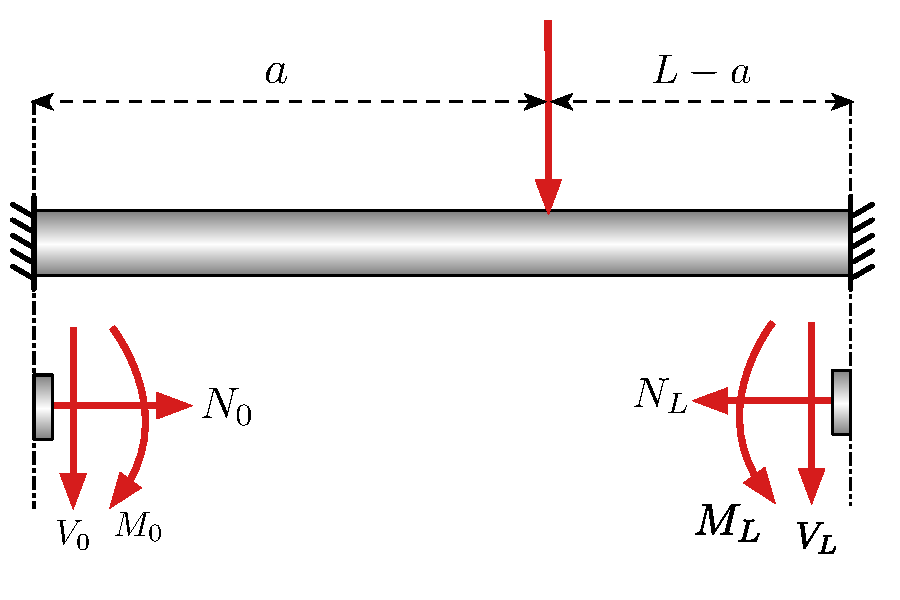
\includegraphics[width=0.5\columnwidth]{Figures/EqPointLoad}}
	\caption{Equivalent Nodal Load}
	\label{fig:EqPointLoad}
\end{figure}
\section{Code}

The structural analysis program will be implemented with an object oriented coding framework. This section will outline how this programming framework is applied to solving structural systems.


\begin{tikzpicture}
\umlclass{StructPy.SturctPy.Node}{
+ x: float\\ 
+ y: float\\ 
+ z: float\\ 
+ fixity: int
}{

}
\end{tikzpicture}

\begin{tikzpicture}
\umlclass{StructPy.SturctPy.Element}{
+
}{
+ length\\
+ element stiffness
}
\end{tikzpicture}




%------------------------------------------------------------------------------------------
\newpage
\bibliography{References}
\addcontentsline{toc}{section}{References}
\bibliographystyle{apalike}

\end{document}